\documentclass[12pt]{article}
\usepackage[utf8]{inputenc}
\usepackage[T2A]{fontenc}
\usepackage[russian]{babel}
\usepackage{amsmath}
\usepackage{amssymb}
\usepackage{dsfont}
\usepackage[dvipsnames]{xcolor}
\usepackage{setspace}
\usepackage{multirow}
\usepackage[a4paper, outer=1.5cm, inner=1.5cm, top=1cm, bottom=1cm]{geometry}
\usepackage{graphicx}
\usepackage{skull}
\usepackage{wasysym}
\usepackage{float}
\graphicspath{{.images/}}
\usepackage{hyperref}
\hypersetup{colorlinks=true, linkcolor=blue, filecolor=magenta, urlcolor=cyan}
\usepackage[firstpage]{draftwatermark}
\SetWatermarkText{
    $\qquad\qquad\qquad\qquad\qquad$\parbox{7cm}{\begin{center}
    
\includegraphics[width = 0.08\textwidth]{lion-logo.png}\bigskip\\~\bigskip\\~\vspace{-24mm}\\~\end{center}}
}
\SetWatermarkAngle{0}
\SetWatermarkScale{1.5}
\usepackage{etoolbox}

\newtoggle{ifsolved}
\newtoggle{needhelp}
\newcounter{num}
\setcounter{num}{1}

\newcommand{\newnum}{\par\textbf{\textnumero\arabic{num}}\stepcounter{num}}
\newcommand{\sol}{\vspace{3mm}\par\textbf{Решение: }}
\newcommand{\ans}{\vspace{3mm}\par\textbf{Ответ: }}
\newcommand{\hint}{\vspace{3mm}\par\textbf{Подсказка: }}
\newcommand{\mode}[1]{
\ifstrequal{#1}{0}{\togglefalse{ifsolved}\togglefalse{needhelp}}{\ifstrequal{#1}{1}{\togglefalse{ifsolved}\toggletrue{needhelp}}{\ifstrequal{#1}{2}{\toggletrue{ifsolved}\togglefalse{needhelp}}{\toggletrue{ifsolved}\toggletrue{needhelp}}}}} %if 0 - if 1 - if 2 - else
%\newenvironment{problem}[8]{%#1, #2, #3
%\parbox{\linewidth}{\vspace{4mm}\ifstrequal{#4}{(лёгкая)}{\newnum\textbf{.}}{\newnum\textbf{*.} } \\ #5}
%\iftoggle{ifsolved}{\sol #6}{}
%\iftoggle{ifsolved}{\ans #7}{}
%\iftoggle{needhelp}{\hint #8}{}}

\newenvironment{problem}[8]{%#1, #2, #3
\parbox{\linewidth}{\vspace{5mm}\ifstrequal{#4}{(лёгкая)}{\newnum\textbf{.}}{\newnum\textbf{*.} } \\ #5}
\iftoggle{ifsolved}{\sol #6}{}

\iftoggle{ifsolved}{\parbox{\linewidth}{\ans #7}}{}
\iftoggle{needhelp}{\parbox{\linewidth}{\hint #8}}{}}

\newenvironment{mylist} %custom list
{ \begin{itemize}
    \setlength{\itemsep}{0pt}
    \setlength{\parskip}{0pt}
    \setlength{\parsep}{0pt}     }
{ \end{itemize}                  }

\newenvironment{homeass}[1]{\vspace*{-1.5cm}
\iftoggle{ifsolved}{
    \section*{\center{Решение домашнего задания к #1.}}
}{
    \section*{\center{\textcolor{Sepia}{Домашнее задание к #1}}}
} \vspace{7mm}\large}

\parindent=0pt
\pagestyle{empty}
%$\!$[\arabic{class}.\arabic{num}]
%\ifnumcomp{\value{counter}}{>}{1}{true}{false}
%\definecolor{Gray}{gray}{0.9}
%\definecolor{mypink}{RGB}{219, 48, 122}
%\newcolumntype{g}{>{\columncolor{Gray}}p{2.8cm}}

\begin{document}
\large
\mode{7}
%0 for problems without hints
%1 for problems + hints
%2 for problems + solutions + answers
%else: show all

{\centering\section*{СПИСОК ЗАДАЧ}}

{\centering\subsection*{\smallskip\\\textcolor{green}{\textbf{Полезные вещи, которые можно и нужно копипастить:}}}}

\subsection*{\textcolor{Emerald}{\textbf{Полезные шпаргалки по LaTeXу:}}}

\textbf{Пример вставки рисунка:}

\begin{minipage}{\linewidth}
    \begin{minipage}{0.54\linewidth}
    см. рисунок справа\\
    Текст к собственно пикче, примерно всегда это либо развёрнутое описание, либо большая часть решения задачи --- стремимся экономить пространство, если это можно сделать.
    \end{minipage}
    \hspace{0.05\linewidth}
    \begin{minipage}{0.4\linewidth}
    \begin{figure}[H] 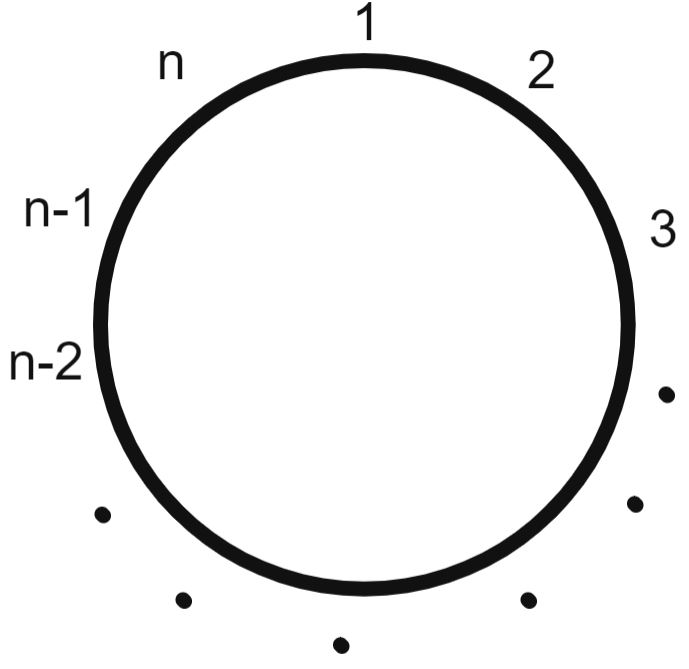
\includegraphics[width=\linewidth]{sol3} %тут поменять имя пикчи
    \end{figure}
    \end{minipage}
\end{minipage}

\textbf{Дефолтные математические знаки и символы:}\\
$\geqslant$,
$\leqslant$,
$a^{b}$,
$x_{i}$,
$\sqrt{a}$,
$\frac{a}{b}$,
$\displaystyle \frac{a}{b}$,
$\cdot$
$\;\Rightarrow\;$,
$\;\Leftrightarrow\;$,
$1{,}2$.
О промежутках:
$a\!b$,
$a\,b$,
$a\:b$,
$a\;b$,
$a\quad b$.

\textbf{Стандартные система и совокупность уравнений / неравенств:}\\
$\left\{
\begin{aligned}
f(x) &= 0 \\
g(x) &= 1
\end{aligned}\right.$

$\left[\begin{aligned}
&\left\{\begin{aligned}
f(x) &\geqslant a \\
g(x) &= b
\end{aligned}\right.\\
&\left\{\begin{aligned}
f(x) &< a \\
g(x) &= -b
\end{aligned}\right.
\end{aligned}\right.$

\subsection*{\textcolor{Emerald}{\textbf{Не математическое, но полезное:}}}
% комментарий в любом месте документа, который нигде не будет видно. Можно использовать для написания заметок-вопросов по задачам
\textbf{Пример таблицы:}

\begin{tabular}{|c|c|c|}
\hline
    $a$ & $b$ & текст
\\\hline
    $c$ & $d$ & мораль
\\\hline
\end{tabular}\\

\textbf{Отступы:} между\smallskip\\ строками\medskip\\ \textbf{Тире} --- это три дефиса.\\
\textbf{Списки:}
\begin{mylist}
\item [$\bullet$] это был пункт а
\item [2)] а это уже пункт номер 2 с изменённым заголовком
\end{mylist}

\subsection*{\textcolor{Emerald}{\textbf{Всё, неупомянутое выше (или если просто что-то не так):}}}
\begin{mylist}
\item [$\bullet$] Решение отдельных вопросов касательно ТеХа нужно искать в \href{https://www.mccme.ru/free-books/llang/newllang.pdf}{Львовском}.

\item [$\bullet$] Найти произвольный символ, который нужен, можно в \href{http://detexify.kirelabs.org/classify.html}{Detexify}.

\item [$\bullet$] Если возникли сомнения при решении, ответ практически ко всем задачам можно проверить с помощью \href{https://www.wolframalpha.com/}{WolframAlpha}.

\item [$\bullet$] Если в задаче нужно создать картинку, то лучше пока отложить эту задачу. Все графики планируется централизованно нарисовать (или перерисовать) в геогебре.

\item [\textcolor{brown}{\textbf{!!}}] Важно ставить \textcolor{red}{\textbf{$\spadesuit$}}
(или просто red) в тело задачи в случае серьёзных вопросов к решению и какой-то вопиющей лажи.

\item [\textcolor{brown}{\textbf{!!}}] Важно ставить \textcolor{olive}{\textbf{$\spadesuit$}}
(или просто olive) в тело задачи в случае не самого удачного текста и кривых отступов.
\end{mylist}

\subsection*{\textcolor{Violet}{\textbf{Комментарии:}}}% а также невидимые комментарии - так можно оставлять заметки-вопросы прямо в задаче, чтобы потом было понятно, в чём вопрос.
\begin{mylist}
\item [$\skull$] Переставлять задачи местами --- очень плохая идея.

\item [$\smiley$] При двойном клике по тексту pdf справа происходит автоматический переход к этому месту в латех-коде, а для обратного перехода можно нажать стрелку вправо (висит сверху между pdf и латех-кодом).

\item [$\smiley$] Если есть размышления, дописывать red/olive к задаче или не дописывать, то лучше всё-таки дописать.

\item [$\skull$] Самое плохое, что можно сделать --- написать в любое поле из трёх (НаписанноеРешение/ВерныйОтвет/Подсказка) только половину того, что надо, никак это не отметить, и потом пойти дальше.\\ Нужно в этот момент писать red/olive в случайном месте задачи, чтобы потом вычислить это с помощью Ctrl+F по всему документу (и это то, что потом будет делаться долго и тщательно)
\end{mylist}

\newpage
\setcounter{num}{1677}

\hypertarget{11.2}{{\centering\section*{\bigskip\\\textcolor{Blue}{\hyperlink{start2}{\textcolor{Blue}{11.2}} Показательная и логарифмическая функции.}\vspace{-5mm}}}}

\begin{problem}{Показательная функция, её свойства и график.}{11.2.1}{9D olive}{(лёгкая)}
{В пруду цветёт одна кувшинка. Каждый день число цветущих кувшинок удваивается, а через 32 дня весь пруд окажется полностью заполнен цветущими кувшинками. Через сколько дней кувшинками будет заполнена четверть пруда?}
{Так как кувшинки увеличиваются вдвое каждый день, значит через 31 день пруд заполнился на половину, потому что на следующий день он удвоился и заполнился полностью. А если через 31 день была заполнена половина, значит днем ранее была заполнена четверть пруда. Следовательно, через 30 дней пруд был заполнен на четверть.}
{Пруд был заполнен на четверть через 30 дней.}{Если за 32 дня пруд заполнился полностью, значит днем ранее пруд был заполнен на половину.}
\end{problem}

\begin{problem}{Показательная функция, её свойства и график.}{11.2.1}{9D olive}{(лёгкая)}
{В результате техногенной катастрофы каждые 10 лет число особей голубого кита сокращается вдвое. Допустим, известно, что в 2015 году их было 12288.\\ Через сколько лет их станет 384?}
{Условие задачи можно записать одним уравнением:\\
$12888\cdot(\frac{1}{2})^{\frac{x}{10}} = 384$, где $x$~--- это количество прошедших лет с 2015 года.\\ Разделим обе части на $12888$, получим: $(\frac{1}{2})^{\frac{x}{10}} = \frac{1}{32} = (\frac{1}{2})^5 $.\\ В силу монотонности показательной функции $\frac{x}{10} = 5 \;\Rightarrow\; x = 50$.}
{Количество особей голубого кита снизится до 384 через 50 лет.}{Закон уменьшения количества особей голубого кита может быть записан как $12888\cdot\left(\frac{1}{2}\right)^\frac{\text{кол-во лет}}{10}$.}
\end{problem}

\begin{problem}{Показательные уравнения.}{11.2.2}{9D}{(лёгкая)}
{Нарисовать графики функций $\displaystyle y = 3^{t}$ и $\displaystyle y = 3^{-t}$.\\ Решить уравнения $\displaystyle \,3^{t} = 729$ и $\displaystyle \,3^{-t} = 9$.}
{НаписанноеРешение}
{ВерныйОтвет}{Подсказка}
\end{problem}

\begin{problem}{Показательные уравнения.}{11.2.2}{9D}{(лёгкая)}
{Решить уравнение $\,4^{x^{2} - 7x + 12} = 16$.}
{Представим $16$, как $4^2$, то есть $4^{x^{2}-7x+12} = 4^2$. В силу монотонности, показательные функции с одинаковыми основаниями равны тогда, когда равны их показатели. Таким образом, получаем, что $x^2-7x+12 = 2$.\\ Переносим $2$ в левую часть: $x^2-7x+10 = 0$. Решая квадратное уравнение, получим два корня: $x = 2$ и $x = 5$.}
{Уравнение имеет два корня: $x = 2$ и $x = 5$.}{Представь $16$, как $4^2$.}
\end{problem}

\begin{problem}{Показательные уравнения.}{11.2.2}{9D}{(лёгкая)}
{Решить уравнение $\,\displaystyle 9^{x} + 6^{x} - 2 \cdot 2^{2x} = 0$.}
{Представим данное уравнение в следующем виде:\\
$9^x+6^x-2\cdot2^{2x} = 3^{2x}+3^x\cdot2^x-2\cdot2^{2x}$. Так как показательная функция строго больше 0, то разделим обе части уравнения на $2^{2x}$: получаем, что\\
$\frac{3^{2x}}{2^{2x}}+\frac{3^x}{2^x}-2 = (\frac{3}{2})^{2x}+(\frac{3}{2})^x-2 = 0$.\\ Сделаем замену $(\frac{3}{2})^x = t$, уравнение сводится к квадратному: $t^2+t-2 = 0$.\\ По теореме Виета находим корни: $t = -2$ и $t = 1$. Делаем обратную замену:\\
$(\frac{3}{2})^x = -2 \;\Rightarrow\;$ вещественных корней нет.\\
$(\frac{3}{2})^x = 1 \;\Rightarrow\; x = 0$.}
{Уравнение имеет единственное вещественное решение $x = 0$.}{Раздели уравнение на $2^{2x}$.}
\end{problem}

\begin{problem}{Показательные уравнения.}{11.2.2}{9D}{(лёгкая)}
{Решить уравнение: $\,\displaystyle 0{,}04^{2 - \sqrt{x - 1}} = 25$.}
{Представим $0,04^{2-\sqrt{x-1}}$, как $(\frac{1}{25})^{2-\sqrt{x-1}} = 25^{\sqrt{x-1}-2}$. Тогда в силу монотонности показательной функции уравнение имеет решение, если показатели степеней равны, то есть если $\sqrt{x-1}-2 = 1 \;\Rightarrow\; \sqrt{x-1} = 3 \;\Rightarrow\; x = 10$.}
{Данное уравнение имеет единственное решение $x = 10$.}{$0,04 = \frac{1}{25}$.}
\end{problem}

\begin{problem}{Показательные уравнения.}{11.2.2}{9D}{(лёгкая)}
{Решить уравнение: $\,\displaystyle 3^{x^{2} - 5x + \frac{7}{2}} = \sqrt{3} \cdot \frac{1}{3^{x}}$.}
{Представим правую часть в виде $\sqrt{3}\cdot\frac{1}{3^x} = 3^{\frac{1}{2}}\cdot3^{-x} = 3^{\frac{1}{2}-x}$. Тогда в силу монотонности показательной функции уравнение имеет решение, если $x^2-5x+\frac{7}{2} = \frac{1}{2}-x$. Перенесем правую часть влево и приведем подобные слагаемые:\\
$x^2-5x+\frac{7}{2}-\frac{1}{2}+x = x^2-4x+3 = 0 \;\Rightarrow\;$ по т. Виета: $x = 1$ и $x = 3$.}
{Уравнение имеет два корня: $x = 1$ и $x = 3$.}{Представь правую часть уравнения как показательную функцию с основанием $3$.}
\end{problem}

\begin{problem}{Показательные уравнения.}{11.2.2}{9D}{(лёгкая)}
{Решить уравнение: $\,\displaystyle \sqrt{5} \cdot 0{,}2^{\frac{1}{2x}} - 0{,}04^{1 - x} = 0$.}
{Перенесём $0,04^{1-x}$ направо и преобразуем обе части уравнения:\\
$5^{\frac{1}{2}}\cdot5^{-\frac{1}{2x}} = (\frac{1}{25})^{1-x} \;\Rightarrow\; 5^{\frac{1}{2}-\frac{1}{2x}} = 5^{-2(1-x)}$. В силу монотонности показательной функции уравнение имеет решение, если $\frac{1}{2}-\frac{1}{2x} = -2+2x$. Перенесем правую часть влево: приходим к уравнению $-2x-\frac{1}{2x}+\frac{1}{2}+2 = 0$. Домножаем на $-2x$:\\
$ \Rightarrow\; 4x^2-5x+1 = 0$. Решаем квадратное уравнение, получаем $x = 1$ и $x = \frac{1}{4}$.}
{Уравнение имеет два решения: $x = 1$ и $x = \frac{1}{4}$.}{Представь оба члена как показательную функцию по основанию $5$.}
\end{problem}

\begin{problem}{Показательные уравнения.}{11.2.2}{9D}{(лёгкая)}
{Решить уравнение: $\displaystyle\, 25^{x} + 1\!\underbrace{00\ldots0}_{x \text{ нулей}} = 2^{2x + 1}$.}
{НаписанноеРешение}
{ВерныйОтвет}{Подсказка}
\end{problem}

\begin{problem}{Показательные уравнения.}{11.2.2}{9D}{(лёгкая)}
{Решить уравнение: $\displaystyle\, 5^{x - 1} + 5 \cdot 0{,}2^{x - 2} = 26$.}
{НаписанноеРешение}
{ВерныйОтвет}{Подсказка}
\end{problem}

\begin{problem}{Показательные уравнения.}{11.2.2}{9D}{(лёгкая)}
{Решить уравнение: $\displaystyle\, 2^{\frac{1}{\sqrt{x} - 1}} \cdot 0{,}5^{\frac{1}{\sqrt{x} + 1}} = 4^{\frac{\sqrt{x}}{x + \sqrt{x}}}$.}
{Поскольку в уравнении участвует корень, первым делом выпишем ОДЗ: $x > 0$, $x \neq 1$. Теперь приводим все экспоненты к одному основанию, в данном случае логично приводить к основанию 2: $\;\displaystyle\, 2^{\frac{1}{\sqrt{x} - 1}} \cdot 0{,}5^{\frac{1}{\sqrt{x} + 1}} = 4^{\frac{\sqrt{x}}{x + \sqrt{x}}} \;\Rightarrow $ \\ $\;\displaystyle\, 2^{\frac{1}{\sqrt{x} - 1}} \cdot \left(2^{-1}\right)^{\frac{1}{\sqrt{x} + 1}} = \left(2^2\right)^{\frac{\sqrt{x}}{x + \sqrt{x}}} \;\Rightarrow \; 2^{\frac{1}{\sqrt{x} - 1}} \cdot 2^{-\frac{1}{\sqrt{x} + 1}} = 2^{\frac{2\sqrt{x}}{x + \sqrt{x}}} \;\Rightarrow\; 2^{\frac{1}{\sqrt{x} - 1} -\frac{1}{\sqrt{x} + 1}} = 2^{\frac{2\sqrt{x}}{x + \sqrt{x}}}$.\\
Так как $2^x$~--- монотонная функция, переходим к равенству показателей степеней.\\ Получаем иррациональное уравнение $\,\displaystyle \frac{1}{\sqrt{x} - 1} -\frac{1}{\sqrt{x} + 1} = \frac{2\sqrt{x}}{x + \sqrt{x}}$, решаем его:\\
$\,\displaystyle \frac{1}{\sqrt{x}\! -\! 1} -\frac{1}{\sqrt{x}\! +\! 1} = \frac{2\sqrt{x}}{x + \sqrt{x}} \;\Rightarrow\; \frac{2}{x - 1} = \frac{2\sqrt{x}}{x + \sqrt{x}} \;\Rightarrow\; \frac{2x + 2\sqrt{x} - 2x\sqrt{x} + 2\sqrt{x}}{(x - 1)(x + \sqrt{x})} = 0$\smallskip\\
$\Rightarrow\; 2x - 2x\sqrt{x} + 4\sqrt{x} = 0 \;\Rightarrow 2\sqrt{x}\,(\sqrt{x} - x + 2) = 0 \;\Rightarrow\; 2\sqrt{x}\,(\sqrt{x} + 1)(2 - \sqrt{x}) = 0$.
Следовательно, подходят $x = 0$ и $x = 4$ (вторая скобка всегда положительна). Однако, $x = 0$ не входит в ОДЗ: в таком случае дробь, являющаяся показателем в правой части исходного уравнения, не будет определена.\\ Поэтому решение только одно~--- $x = 4$.}
{Данное показательное уравнение имеет один корень, $x = 4$.}{Все экспоненты надо вначале привести к общему основанию.}
\end{problem}

\begin{problem}{Показательные уравнения.}{11.2.2}{10A}{(лёгкая)}
{Решить уравнение: $\,2^{z} \cdot 5^{z - 1} = 200$.}
{НаписанноеРешение}
{ВерныйОтвет}{Подсказка}
\end{problem}

\begin{problem}{Показательные неравенства.}{11.2.3}{9D}{(лёгкая)}
{Решить неравенство: $\,\displaystyle 3^{x - 2} \leqslant \frac{1}{3}$.}
{НаписанноеРешение}
{ВерныйОтвет}{Подсказка}
\end{problem}

\begin{problem}{Показательные неравенства.}{11.2.3}{9D}{(лёгкая)}
{Решить неравенство: $\,\displaystyle \left(\frac{1}{2}\right)^{\!x} \!< \,\frac{1}{8}$.}
{НаписанноеРешение}
{ВерныйОтвет}{Подсказка}
\end{problem}

\begin{problem}{Показательные неравенства.}{11.2.3}{9D}{*}
{Решить неравенство: $\,(x - 2)^{1 - x} \geqslant 1$.}
{НаписанноеРешение}
{ВерныйОтвет}{Подсказка}
\end{problem}

\begin{problem}{Показательные неравенства.}{11.2.3}{9D}{(лёгкая)}
{Решить неравенство: $\displaystyle \,4^{x + \frac{1}{x}} \geqslant 32$.}
{НаписанноеРешение}
{ВерныйОтвет}{Подсказка}
\end{problem}

\begin{problem}{Показательные неравенства.}{11.2.3}{9D}{(лёгкая)}
{Решить неравенство: $\displaystyle \,2^{1 - 2^{\frac{1}{x}}} \leqslant 0{,}125$.}
{НаписанноеРешение}
{ВерныйОтвет}{Подсказка}
\end{problem}

\begin{problem}{Показательные неравенства.}{11.2.3}{9D}{(лёгкая)}
{Решить неравенство: $\displaystyle \,\left(\!\left(\frac{3}{7}\right)^{\!\!\frac{1}{x^{2}}}\right)^{\!\!x^{2} - 2x} \!\!\!\geqslant \text{\LARGE \raisebox{-2pt}{1.}}$}
{При возведении степени в степень степени перемножаются.\\ Поэтому получаем неравенство $\displaystyle \left(\frac{3}{7}\right)^{\!\! 1 - \frac{2}{x}} \!\!\geqslant \text{\LARGE \raisebox{-2pt}{1}} \;\Rightarrow\; \left(\frac{3}{7}\right)^{\!\! 1 - \frac{2}{x}} \!\!\geqslant \left(\frac{3}{7}\right)^{\!\!0}$.\\ В нашем показательном неравенстве основания степеней равны $\frac 37$, что меньше 1. Поэтому когда мы переходим к сравнению показателей степеней, знак неравенства меняется $\;\Rightarrow\;  1 - \frac 2x \leqslant 0 \;\Rightarrow\; \frac{x - 2}{x} \leqslant 0$. Решаем данное рациональное неравенство при помощи метода интервалов: получаем, что $x \in (0; 2]$.}
{Решением показательного неравенства является полуинтервал $(0; 2]$.}{Что происходит при возведении степени в степень?}
\end{problem}

\begin{problem}{Показательные неравенства.}{11.2.3}{9D}{(лёгкая)}
{Решить неравенство: $\,\displaystyle 4^{x} - 10 \cdot 2^{x - 1} - 24 \leqslant 0$.}
{НаписанноеРешение}
{ВерныйОтвет}{Подсказка}
\end{problem}

\begin{problem}{Показательные неравенства.}{11.2.3}{9D}{(лёгкая)}
{Решить неравенство: $\,\displaystyle 10^{1 + x^{2}} - 10^{1 - x^{2}} \geqslant 99$.}
{НаписанноеРешение}
{ВерныйОтвет}{Подсказка}
\end{problem}

\begin{problem}{Показательные неравенства.}{11.2.3}{9D}{(лёгкая)}
{Решить неравенство: $\displaystyle\, 0{,}6^{x} \cdot \left(\frac{25}{9}\right)^{\!\!x^{2} - 12} \!\!\!< \left(\frac{27}{125}\right)^{\!\!3}$.}
{НаписанноеРешение}
{ВерныйОтвет}{Подсказка}
\end{problem}

\begin{problem}{Показательные неравенства.}{11.2.3}{9D}{(лёгкая)}
{Решить неравенство: $\,\displaystyle 8^{\frac{x - 3}{3x - 7}} \cdot \sqrt[3]{\!\sqrt{0{,}25^{\frac{3x - 1}{x - 1}}}} \leqslant \;\text{\LARGE \raisebox{-2pt}{1.}}$}
{НаписанноеРешение}
{ВерныйОтвет}{Подсказка}
\end{problem}

\begin{problem}{Свойства логарифмов.}{11.2.5}{9D red многопунктовая}{(лёгкая)}
{Вычислить:
\\a) $\displaystyle \lg8 - \lg0{,}0016 - \lg5 =$
\\b) $\displaystyle \log_{0{,}2}40 + \log_{0{,}2}3{,}125 =$
\\c) $\displaystyle \log_{\sqrt{7}}(\sqrt{3} + \sqrt{2}) + \log_{\sqrt{7}}(\sqrt{3} - \sqrt{2}) =$
\\d) $\displaystyle \log_{3}75 - \log_{3}(7 - 2\sqrt{6}) - \log_{3}(7 + 2\sqrt{6}) =$
\\e) $\displaystyle \log_{3}40 + \log_\frac{1}{3}120 =$}
{a) $\lg8 - \lg0{,}0016 - \lg5 = \lg(2^3) - \lg(2^4 \cdot 10^{-4}) - \lg5 = 3\lg2 - (\lg2^4 + \lg(10^{-4})) - \lg5 = 3\lg2 - 4\lg2 - (-4)\lg10 - \lg5 = -\lg2 - \lg5 + 4 = -(\lg(2 \cdot 5)) + 4 = -\lg10 + 4 = 3$. \\
b) $\log_{0{,}2}40 + \log_{0{,}2}3{,}125 = \log_{\frac{1}{5}}(5 \cdot 8) + \log_{\frac{1}{5}}(5^5 \cdot 10^{-3}) = \log_{5^{-1}}5 + \log_{5^{-1}}8 + \log_{5^{-1}}(5^5) + \log_{5^{-1}}(10^{-3}) = -\log_{5}5 - \log_{5}(2^3) - 5\log_{5}5 -\log_{5}(5^{-3} \cdot 2^{-3}) = -1 -3\log_{5}2 - ((-3)\log_{5}5 + (-3)\log_{5}2) =  -1 -3\log_{5}2 + 3\log_{5}5 + 3\log_{5}2 = 2$. \\
c) $\log_{\sqrt{7}}(\sqrt{3} + \sqrt{2}) + \log_{\sqrt{7}}(\sqrt{3} - \sqrt{2}) = \log_{\sqrt{7}}((\sqrt{3} + \sqrt{2})(\sqrt{3} - \sqrt{2})) = \log_{\sqrt{7}}1 = 0$.\\
d) $\log_{3}75 - \log_{3}(7 - 2\sqrt{6}) - \log_{3}(7 + 2\sqrt{6}) = \log_{3}(5^2 \cdot 3) - (\log_{3}(7 - 2\sqrt{6}) + \log_{3}(7 + 2\sqrt{6})) = 2\log_{3}5 + \log_{3}3 - \log_{3}((7 - 2\sqrt{6})(7 + 2\sqrt{6})) = 2\log_{3}5 + 1 - \log_{3}25 = 1$. \\
e) $ \log_{3}40 + \log_\frac{1}{3}120 = \log_{3}40 + \log_{3^{-1}}(40 \cdot 3) = \log_{3}40 + (-1)\log_{3}40 + (-1)\log_{3}3 = -1$.}
{a) 3; b) 2; c) 0; d) 1; e) -1.}{Используем основные свойства логарифмов.}
\end{problem}

\begin{problem}{Логарифмические уравнения.}{11.2.6}{9D}{(лёгкая)}
{Решить уравнение $\,\displaystyle \log_{10}\!\left(\!x + \frac{3}{2}\right) = -\log_{10} x$.}
{Поскольку логарифм определён только для положительных значений, выпишем ОДЗ: $\,\begin{cases}
x + \frac{3}{2} > 0 \\
\;\;\,x > 0
\end{cases} \!\!\!\Rightarrow\; x > 0$.
Перенесём все логарифмы в левую часть уравнения и используем, что сумма логарифмов равна логарифму произведения,\\ получаем:
$\,\displaystyle \log_{10}\!\left(\!x + \frac{3}{2}\right) = -\log_{10} x \;\Rightarrow\; \log_{10}\!\left(\!x^2 + \frac{3}{2}x\right) = 0 = \log_{10} 1$. В силу монотонности логарифма переходим к равенству подлогарифменных выражений:\smallskip\\ $x^2 + \frac{3}{2}x = 1 \;\Rightarrow\; x^2 + \frac 32 x - 1 = 0 \;\Rightarrow\; (x + 2)(x - \frac 12) = 0 \;\Rightarrow\; x = -2;\, x = \frac12$.\\
Учитываем ОДЗ, в результате чего остаётся только один корень $x = \frac12$.\\ Проверка: $\log_{10} 2 = -\log_{10} \frac12$, всё верно.}
{Решением данного логарифмического уравнения является $x = \frac12$.}{Чему равна сумма логарифмов?}
\end{problem}

\begin{problem}{Логарифмические уравнения.}{11.2.6}{9D}{(лёгкая)}
{Решить уравнение $\,\displaystyle \log_2(x - 1) = \log_2 7 - \log_2(x + 5)$.}
{Поскольку логарифм определён только для положительных значений, выпишем ОДЗ: $\,x - 1 > 0$ и $x + 5 > 0 \;\Rightarrow\; x > 1$.\smallskip\\ Теперь решим логарифмическое уравнение: вначале перенесём все логарифмы в левую часть уравнения, а потом воспользуемся свойствами логарифмов:\\
$\displaystyle \log_2(x - 1) = \log_2 7 - \log_2(x + 5) \;\Rightarrow\; \log_2(x - 1) - \log_2 7 + \log_2(x + 5) = 0 \;\Rightarrow\;$ \\
$\log_2\!\left(\!\frac{(x - 1)(x + 5)}{7}\!\right) = 0 \;\Rightarrow\; \log_2\!\left(\!\frac{(x - 1)(x + 5)}{7}\!\right) = \log_2 1$. Поскольку логарифм является монотонной функцией, подлогарифменные выражения равны. Следовательно,\\
$\frac{(x - 1)(x + 5)}{7} = 1 \;\Rightarrow\; x^2 + 4x - 5 = 7 \;\Rightarrow\; x^2 + 4x - 12 = 0 \;\Rightarrow\; (x - 2)(x + 6) = 0$.\\
Таким образом, мы получили два корня: $x = -6$ и $x = 2$.\\ Однако, ОДЗ~--- $x > 1$, поэтому $x = -6$ является посторонним корнем, а решением уравнения является только $x = 2$.}
{Решением логарифмического уравнения является $x = 2$.}{Используй свойства логарифмов.}
\end{problem}

\begin{problem}{Логарифмические уравнения.}{11.2.6}{9D}{(лёгкая)}
{Решить уравнение $\displaystyle\, \log_5 (3x - 11) + \log_5 (x - 27) = 3 + \log_5 8$.}
{Вначале выпишем ОДЗ: $3x - 11 > 0$, $x - 27 > 0 \;\Rightarrow\; x > \frac{11}{3}$ и $x > 27$.\\ Следовательно, $x > 27$. $\;$ Сумма логарифмов равна логарифму произведения: $\displaystyle\, \log_5 (3x - 11) + \log_5 (x - 27) = 3 + \log_5 8 \;\Rightarrow\; \log_5 \left((3x - 11)(x - 27)\right) = \log_5 \left(5^3 \cdot 8\right) \;\Rightarrow$\\ $\Rightarrow\; \log_5 (3x^2 - 92x + 297) = \log_5 1000 \;\Rightarrow\; 3x^2 - 92x + 297 = 1000 \;\Rightarrow$ \\ $\Rightarrow\; 3x^2 - 92x - 703 = 0$. Решаем квадратное уравнение через дискриминант: $D = 92^2 - 4 \cdot 3 \cdot (-703) = 4 \cdot 46^2 + 4 \cdot 2109 = 4 \cdot (2116 + 2109) = 4 \cdot 4225 = 16900 = 130^2$ \\ $\displaystyle \Rightarrow\; x_{1,2} = \frac{92 \pm 130}{6} = 37; -\frac{19}{3}$.\\ В ОДЗ находятся только $x > 27$, поэтому $x = -\frac{19}{3}$~--- посторонний корень.}
{$x = 37$.}{ОДЗ! Дискриминант должен в итоге быть точным квадратом.}
\end{problem}

\begin{problem}{Логарифмические уравнения.}{11.2.6}{9D}{(лёгкая)}
{Решить уравнение $\displaystyle\, \lg (5 - x) + 2\lg \sqrt{3 - x} = 1$.}
{Первым делом выпишем ОДЗ: $5 - x > 0$ и $3 - x > 0$ $\;\Rightarrow\; x < 3$.\\ Cумма логарифмов равна логарифму произведения, следовательно:\\
$\displaystyle\, \lg (5 - x) + 2\lg \sqrt{3 - x} = \lg (5 - x)(3 - x) = 1 \;\Rightarrow\; \lg (5 - x)(3 - x) = \lg 10$.\\
Поскольку логарифм является монотонной функцией, получаем квадратное уравнение $(5 - x)(3 - x) = 10$. Решаем его: $15 - 8x + x^2 = 10 \;\Rightarrow\; x^2 - 8x + 5 = 0 \; \Rightarrow\;$ \\
$\displaystyle D = 64 - 20 = 44 \;\Rightarrow\; x = \frac{8\pm2\sqrt{11}}{2} = 4\pm\sqrt{11}$.\\ Учитывая что $4 + \sqrt{11} > 3$, это посторонний корень, не входящий в ОДЗ.\\ Поэтому решение у данного уравнения только одно~--- $x = 4 - \sqrt{11}$.}
{$x = 4 - \sqrt{11}$.}{Логарифм произведения есть сумма логарифмов.\\ В ходе решения не забыть проверить ОДЗ.}
\end{problem}

\begin{problem}{Логарифмические уравнения.}{11.2.6}{9D}{(лёгкая)}
{Решить уравнение $\displaystyle\, \lg (5 - x) = \frac 13 \lg (35 - x^3)$.}
{Выпишем ОДЗ: $5 - x > 0 \Rightarrow x < 5$, $35 - x^3 > 0 \Rightarrow x^3 < 35 \Rightarrow x < \sqrt[3]{35}$. Таким образом, $x < \sqrt[3]{35}$. Преобразуем наше выражение:\\ $\lg (5 - x) = \frac 13 \lg (35 - x^3) \;\Rightarrow\; 3\lg (5 - x) = \lg (35 - x^3)$.\\ В силу монотонности логарифма, приходим к уравнению $(5 - x)^3 = 35 - x^3 \;\Rightarrow\; 125 - 75x + 15x^2 - x^3 = 35 - x^3 \;\Rightarrow\; 90 - 75x + 15x^2 = 0 \;\Rightarrow\; x^2 - 5x + 6 = 0 \;\Rightarrow\; $\\
$(x - 3)(x - 2) = 0 \;\Rightarrow\; x = 2$, $x  = 3$.\\ Оба корня подходят ($\sqrt[3]{35} > \sqrt[3]{27} = 3 > 2$) и не являются посторонними.}
{Данное логарифмическое уравнение имеет два корня: $x = 2$ и $x = 3$.}{Воспользоваться свойствами суммы логарифмов и монотонностью логарифма. В ходе решения не забыть проверить ОДЗ.}
\end{problem}

\begin{problem}{Логарифмические уравнения.}{11.2.6}{9D}{(лёгкая)}
{Решить уравнение $\displaystyle\, \log_2 182 - 2\log_2 \sqrt{5 - x} = \log_2 (11 - x) + 1$.}
{НаписанноеРешение}
{ВерныйОтвет}{Подсказка}
\end{problem}

\begin{problem}{Логарифмические уравнения.}{11.2.6}{9D}{(лёгкая)}
{Решить уравнение $\displaystyle\, \log_5 \sqrt{x - 9} - \log_5 10 + \log_5 \sqrt{2x - 1} = 0$.}
{В первую очередь проверим ОДЗ: $\left\{\begin{aligned}
x - 9 > 0\\
10 > 0\\
2x - 1 > 0
\end{aligned}\right. \;\Rightarrow\; x > 9$.\\
Собираем все логарифмы в один: $\displaystyle \log_5 \left(\frac{\sqrt{x - 9}\sqrt{2x - 1}}{10}\right) = \log_5 1$.\\ Используем монотонность $\;\Rightarrow\;\displaystyle \frac{\sqrt{x - 9}\sqrt{2x - 1}}{10} = 1 \;\Rightarrow\; \sqrt{(x - 9)(2x - 1)} = 10$ \\
$\Rightarrow\; 2x^2 - 19x + 9 = 100 \;\Rightarrow\; 2x^2 - 19x - 91 = 0$. $D = 19^2 + 8\cdot91 = 1089 = 33^2 \;\Rightarrow$\\
$\Rightarrow x = \frac{19\pm33}{4} = -\frac72$, $13.\,$ Согласно ОДЗ $x > 9$, остаётся только корень $x = 13$.}
{$x = 13$.}{Сумма/разность логарифмов является логарифмом произведения/частного. Логарифм с любым основанием от 1 равен 0.}
\end{problem}

\begin{problem}{Логарифмические уравнения.}{11.2.6}{9D}{(лёгкая)}
{Решить уравнение $\displaystyle\, \log_2\frac{x - 5}{x + 5} + \log_2 (x^{2} - 25) = 0$.}
{НаписанноеРешение}
{ВерныйОтвет}{Подсказка}
\end{problem}

\begin{problem}{Логарифмические уравнения.}{11.2.6}{9D}{(лёгкая)}
{Решить систему уравнений:
$\quad\displaystyle \left\{\begin{aligned}
    3^{y} &\cdot 9^{x} = 81 \\
    \lg (x + y)^{2} &- \lg x = 2\lg3
\end{aligned}\right.$.}
{НаписанноеРешение}
{ВерныйОтвет}{Подсказка}
\end{problem}

\begin{problem}{Логарифмические уравнения.}{11.2.6}{9D}{(лёгкая)}
{Решить уравнение $\displaystyle\, \log_6 \left(3^{x^2} + 1\right) - \log_6 \left(3^{2 - x^2} + 9\right) = \log_6 2 - 1$.}
{НаписанноеРешение}
{ВерныйОтвет}{Подсказка}
\end{problem}

\begin{problem}{Логарифмические уравнения.}{11.2.6}{9D}{(лёгкая)}
{Решить уравнение $\displaystyle \log_3\!\left(3^{x^2 - 13x + 28} + \frac29\right) = \log_5 0{,}2$.}
{Поскольку подлогарифменное выражение представляет собой сумму экспоненты и положительного числа, ОДЗ не накладывает никаких ограничений на $x$. Отметим, что второй логарифм равен $\log_5 \frac15 = -1$.\\ Таким образом, $\displaystyle \log_3\!\left(3^{x^2 - 13x + 28} + \frac29\right) = -1 \;\Rightarrow\; \log_3\!\left(3^{x^2 - 13x + 28} + \frac29\right) = \log_3 \frac13$.\\
В силу монотонности логарифма $\displaystyle 3^{x^2 - 13x + 28} + \frac29 = \frac13 \;\Rightarrow\; 3^{x^2 - 13x + 28} = \frac19 = 3^{-2}$.\\
В силу монотонности экспоненты $x^2 - 13x + 28 = -2 \;\Rightarrow\; x^2 - 13x + 30 = 0$.\smallskip\\
Решаем квадратное уравнение через дискриминант: $D = 169 - 120 = 49 = 7^2 \;\Rightarrow\; x = \frac{13\pm7}{2} = 3; 10$. Итого, уравнение имеет два корня~--- $x = 3$ и $x = 10$.}
{Данное логарифмическое уравнение имеет два корня: $x = 3$ и $x = 10$.}{Второй логарифм может быть явно вычислен.}
\end{problem}

\begin{problem}{Логарифмические уравнения.}{11.2.6}{9D}{(лёгкая)}
{Решить уравнение $\displaystyle \log_2 x + \log_4 x + \log_8 x = 11$.}
{НаписанноеРешение}
{ВерныйОтвет}{Подсказка}
\end{problem}

\begin{problem}{Логарифмические уравнения.}{11.2.6}{9D}{(лёгкая)}
{Решить уравнение $\,\log_4(\log_2 x) + \log_2(\log_4 x) = 2$.}
{НаписанноеРешение}
{ВерныйОтвет}{Подсказка}
\end{problem}

\begin{problem}{Логарифмические уравнения.}{11.2.6}{9D}{*}
{Решить уравнение $\displaystyle\, \log_{5}(x - 2) + \log_{\sqrt{5}}(x^{3} - 2) + \log_{0{,}2} (x - 2) = 4$.}
{Поскольку логарифм определён только для положительных значений, найдём ОДЗ: $\,\begin{cases}
x - 2 > 0 \\
x^3 - 2 > 0
\end{cases} \!\!\!\Rightarrow\; x > \sqrt[3]{2}$. Для того, чтобы сложить все логарифмы, приведём их к одному основанию: для этого заметим, что $\sqrt{5} = 5^{\frac12}$, $\,0{,}2 = 5^{-1}$.\\ Из основного логарифмического тождества можно получить, что $\log_{a^k} b = \log_a b^{\frac1k}$, или, что то же самое, $\log_a b = \log_{a^c} b^c$. Поэтому получаем следующее:\\
$\displaystyle\, \log_{5}(x - 2) + \log_{\sqrt{5}}(x^{3} - 2) + \log_{0{,}2} (x - 2) = 4 \;\Rightarrow\; \log_{5}(x - 2) + \log_{5}(x^3 - 2)^2 + \log_{5}(x - 2)^{-1} = 4 \;\Rightarrow\; \log_5 \left((x - 2)(x^3 - 2)^2(x - 2)^{-1}\right) = \log_5 5^4 \;\Rightarrow\; \log_{5}(x^3 - 2)^2 = \log_5 5^4$.\smallskip\\
Из монотонности логарифма получаем равенство подлогарифменных выражений: $(x^3 - 2)^2 = 5^4 \;\Rightarrow\; x^3 - 2 = \pm 25 \;\Rightarrow\; \left[\begin{aligned}
x^3 &= 27\\
x^3 &= -23
\end{aligned}\right. \;\Rightarrow\; \left[\begin{aligned}
x &= 3\\
x &= -\sqrt[3]{23}
\end{aligned}\right.$\smallskip\\
После учёта ОДЗ остаётся только один корень $x = 3$: отрицательный корень~--- посторонний.}
{Решением логарифмического уравнения является $x = 3$.}{Вначале нужно привести все логарифмы к одному основанию.}
\end{problem}

\begin{problem}{Логарифмические уравнения.}{11.2.6}{9D}{(лёгкая)}
{Решить уравнение $\displaystyle \,\log_{3} x \cdot \log_{9} x \cdot \log_{27} x \cdot \log_{81} x = \frac{2}{3}$}
{Для начала отметим, что так как все подлогарифменные выражения равны $x$, то мы имеем следующее ОДЗ: $x > 0$. Для решения этого уравнения заменим основания всех логарифмов на 3: $\displaystyle \,\log_{3} x \cdot \log_{9} x \cdot \log_{27} x \cdot \log_{81} x = \frac{2}{3} \;\Rightarrow\; \log_{3} x \cdot \frac{\log_{3} x}{\log_{3} 9} \cdot \frac{\log_{3} x}{\log_{3} 27} \cdot \frac{\log_{3} x}{\log_{3} 81} = \frac{2}{3} \;\Rightarrow\; \frac{(\log_3 x)^4}{2 \cdot 3 \cdot 4} = \frac23 \;\Rightarrow\; (\log_3 x)^4 = 16$.\\
Сделаем замену $t = \log_3 x$: решаем уравнение $t^4 = 16$.\\ $t^4 = 16 \;\Rightarrow\; \left[\begin{aligned}
t^2 &= -4\\
t^2 &= 4
\end{aligned}\right. \;\Rightarrow\; \left[\begin{aligned}
t &= -2\\
t &= 2
\end{aligned}\right. \;\Rightarrow\; \left[\begin{aligned}
\log_3 x &= -2\\
\log_3 x &= 2
\end{aligned}\right. \;\Rightarrow\; \left[\begin{aligned}
x &= 3^{-2}\\
x &= 3^{2}
\end{aligned}\right. \;\Rightarrow\; x = \frac19;\, 9$.}
{Данное уравнение имеет два корня, $x = \frac19$ и $x = 9$.}{Заменить все основания на одно и то же (например, 3).\\ Сделать замену.}
\end{problem}

\begin{problem}{Логарифмические уравнения.}{11.2.6}{9D}{(лёгкая)}
{Решить уравнение $\displaystyle \,\log_{1 - x} 3 - \log_{1 - x} 2 - 0{,}5 = 0$.}
{НаписанноеРешение}
{ВерныйОтвет}{Подсказка}
\end{problem}

\begin{problem}{Логарифмические уравнения.}{11.2.6}{9D}{(лёгкая)}
{Решить уравнение $\displaystyle \,2\log_{x} 27 - 3\log_{27}x = 1$.}
{Согласно свойству логарифма $\log_a b = \frac{1}{\log_b a}$, мы можем представить $2\log_x 27$, как $\frac{2}{\log_{27} x}$. Сделаем замену $\log_{27} x = t$. Тогда уравнение примет вид:\\
$\frac{2}{t}-3t = 1$. Перенесем правую часть налево и домножим на t:\\
$3t^2+t-2 = 0$. Решаем квадратное уравнение, получаем $t = -1$ и $t = \frac{2}{3}.$\\
1) ${\log_{27} x} = -1 \;\Rightarrow\; x = \frac{1}{27}.$\\
2) ${\log_{27} x} = \frac{2}{3} \;\Rightarrow\; x = 27^{\frac{2}{3}} = 9.$
}
{Уравнение имеет два решения: $x = 9$ и $x = \frac{1}{27}$.}{$\log_a b = \frac{1}{\log_b a}$.}
\end{problem}

\begin{problem}{Логарифмические неравенства.}{11.2.7}{9D}{(лёгкая)}
{Решить неравенство: $\displaystyle \,\log_3 \frac{1}{x} + \log_3 (x^{2} + 3x - 9) \leqslant \log_3 \left(\!x^{2} + 3x + \frac{1}{x} - 10\!\right)$.}
{НаписанноеРешение}
{ВерныйОтвет}{Подсказка}
\end{problem}

\begin{problem}{Логарифмические неравенства.}{11.2.7}{9D}{*}
{Решить неравенство: $\, (\log_x 2 - 1) \log_2 (2x) \leqslant \frac{3}{2}$.}
{Для начала находим ОДЗ: $\left\{\begin{aligned}
2x > 0\\
x > 0\\
x \neq 1
\end{aligned}\right. \;\Rightarrow\; x \in (0; 1) \cup (1; +\infty)$.\smallskip\\
Используем свойства логарифмов: $(\log_x 2 - 1) \log_2 (2x) \leqslant \frac{3}{2} \;\Rightarrow\;\,$ (замена $t = \log_2 x$)\\ $(\frac{1}{\log_2 x} - 1) \cdot (\log_2 2 + \log_2 x) \leqslant \frac{3}{2} \;\Rightarrow\; (\frac1t - 1)(1 + t) \leqslant \frac32 \;\Rightarrow\; \frac{1 - t^2}{t}\leqslant \frac32 \;\Rightarrow\; \frac{2 - 3t - 2t^2}{2t} \leqslant 0$\\
$\Rightarrow\; -\frac{(2t - 1)(t + 2)}{2t} \leqslant 0 \;\Rightarrow\; \frac{(2t - 1)(t + 2)}{2t} \geqslant 0 \;\Rightarrow\; t \in [-2; 0) \cup [\frac12; +\infty)$.\\
Теперь сделаем обратную замену $t = \log_2 x$ и решим получившиеся неравенства:\\
$\left[\begin{aligned}
-2 &\leqslant \log_2 x < 0\\
\frac12 &\leqslant \log_2 x
\end{aligned}\right. \;\Rightarrow\; \left[\begin{aligned}
\log_2 2^{-2} &\leqslant \log_2 x < \log_2 2^{0}\\
\log_2 2^{\frac12} &\leqslant \log_2 x
\end{aligned}\right. \;\Rightarrow\; \left[\begin{aligned}
\frac14 &\leqslant x < 1\\
\sqrt{2} &\leqslant x
\end{aligned}\right. \;\Rightarrow\;$\\
$\Rightarrow\; x \in [\frac14; 1) \cup [\sqrt{2}; +\infty)$.}
{Решением логарифмического неравенства $\, (\log_x 2 - 1) \log_2 (2x) \leqslant \frac{3}{2}$\\ является множество $x \in [\frac14; 1) \cup [\sqrt{2}; +\infty)$.}{Используй свойства логарифмов перед тем как сделать замену.}
\end{problem}

\begin{problem}{Логарифмические неравенства.}{11.2.7}{9D}{*}
{Решить неравенство: $\displaystyle \,\frac{\lg(5y^{2} - 2y + 1)}{\lg(4y^{2} - 5y + 1)^{3}} \leqslant \frac{\log_{5^{3}}7}{\log_{5}7}$.}
{НаписанноеРешение}
{ВерныйОтвет}{Подсказка}
\end{problem}

\begin{problem}{Логарифмические неравенства.}{11.2.7}{9D}{*}
{Решить неравенство: $\displaystyle \,\log_{0{,}5}(x - 3) - \log_{0{,}5}(x + 3) - \log_{\frac{x + 3}{x - 3}} 2 > 0$.}
{В первую очередь находим ОДЗ:\\ $\left\{\begin{aligned}
x - 3 > 0\\
x + 3 > 0\\
\frac{x + 3}{x - 3} > 0\\
\frac{x + 3}{x - 3} \neq 1
\end{aligned}\right.\;\Rightarrow\;\left\{\begin{aligned}
x &> 3\\
\frac{x + 3}{x - 3} &\neq \frac{x - 3}{x - 3}
\end{aligned}\right. \;\Rightarrow\; x > 3\quad$ \parbox{7.5cm}{(второе неравенство не накладывает никаких ограничений, так как эти дроби никогда не равны)}\smallskip\\
Решаем наше неравенство:\\
$\log_{0{,}5}(x - 3) - \log_{0{,}5}(x + 3) - \log_{\frac{x + 3}{x - 3}} 2 > 0 \;\Rightarrow\; \log_{0{,}5} \frac{x - 3}{x + 3} - \log_{\frac{x + 3}{x - 3}} 2 > 0$. Делаем замену $t = \frac{x + 3}{x - 3}$: $\log_{0{,}5} \frac{1}{t} - \log_t 2 > 0 \;\Rightarrow\; \log_{\frac12}\frac1t - \log_t 2 > 0 \;\Rightarrow\; \log_2 t - \log_t 2 > 0$.\smallskip\\
Учитывая, что если $y = \log_a b$, то $\log_b a = \frac1y$, делаем замену $y = \log_2 t$:\\
$\displaystyle y - \frac1y > 0 \;\Rightarrow\; \frac{(y - 1)(y + 1)}{y} > 0 \;\Rightarrow\; y \in (-1; 0) \cup (1; +\infty)$.\\ Сделаем обратную замену $y = \log_2 t\,$ и найдём, в каких пределах меняется $t$:\\
$\left[\begin{aligned}
-1 &< \log_2 t < 0\\
1 &< \log_2 t
\end{aligned}\right. \;\Rightarrow\; \left[\begin{aligned}
\log_2 2^{-1} &< \log_2 t < \log_2 2^{0}\\
\log_2 2^{1} &< \log_2 t
\end{aligned}\right. \;\Rightarrow\; \left[\begin{aligned}
\frac12 &< t < 1\\
2 &< t
\end{aligned}\right.$\\
Таким образом, $t \in (\frac12; 1) \cup (2; +\infty)$. Теперь вторая обратная замена, $t = \frac{x + 3}{x - 3}$:\\
$\left[\begin{aligned}
\frac12 &< \frac{x + 3}{x - 3} < 1\\
2 &< \frac{x + 3}{x - 3}
\end{aligned}\right. \;\Rightarrow\; \left[\begin{aligned}
x \in \varnothing\; &(\text{в ОДЗ})\\
\frac{2x - 6}{x - 3} &< \frac{x + 3}{x - 3}
\end{aligned}\right. \;\Rightarrow\; \displaystyle \frac{x - 9}{x - 3} < 0 \;\Rightarrow\; x \in (3; 9)$.}
{Решением данного неравенства является интервал $(3; 9)$.}{После применения свойств логарифмов можно заметить выражение, для которого нужно сделать замену. Можно решать и в два шага, сделав две упрощающие замены по очереди. В ходе решения полезно помнить про ОДЗ: конкретно в данном случае это может существенно упростить решение!}
\end{problem}

\begin{problem}{Логарифмические неравенства.}{11.2.7}{9D}{(лёгкая)}
{Решить систему неравенств:
$\quad\left\{\begin{aligned}
    (x - 1)\lg 2 + \lg (2^{x + 1} + 1) &< \lg (7 \cdot 2^{x} + 12)\\
    \log_x (x + 2) &> 2.
\end{aligned}\right.$}
{НаписанноеРешение}
{ВерныйОтвет}{Подсказка}
\end{problem}

\begin{problem}{Логарифмические неравенства.}{11.2.7}{9D}{(лёгкая)}
{Решить неравенство: $\,\log_5(4 + x) \leqslant 3$.}
{НаписанноеРешение}
{ВерныйОтвет}{Подсказка}
\end{problem}

\begin{problem}{Логарифмические неравенства.}{11.2.7}{9D}{(лёгкая)}
{Решить неравенство: $\,\log_{0{,}5}(x - 9) > -4$.}
{Выпишем ОДЗ: $x - 9 > 0 \;\Rightarrow\; x > 9$.\smallskip\\
$\,\log_{0{,}5}(x - 9) > -4 \;\Rightarrow\; \log_{0{,}5}(x - 9) > \log_{0{,}5} \left(\frac12\right)^{-4}$. При основании $a \in (0; 1)$ знак неравенства меняется на противоположный: $x - 9 < \left(\frac12\right)^{-4} \;\Rightarrow\; x < 9 + 16 = 25$.\\
Учитывая ОДЗ, получаем $x \in \left(9; 25\right)$.}
{Решением неравенства $\,\log_{0{,}5}(x - 9) > -4$ является интервал $\left(9; 25\right)$.}{Когда меняется знак в логарифмических неравенствах?}
\end{problem}

\begin{problem}{Логарифмические неравенства.}{11.2.7}{9D}{(лёгкая)}
{Решить неравенство: $\,\displaystyle \log_3\frac{3x - 5}{x + 1} \leqslant 1.$}
{Первым делом проверяем ОДЗ: $\displaystyle\,\frac{3x - 5}{x + 1} > 0 \;\Rightarrow\;$ (согласно методу интервалов) $\;\Rightarrow\; x \in (-\infty; -1) \cup (\frac53; +\infty)$. Теперь можно решать наше неравенство:\smallskip\\ $\,\displaystyle \log_3\frac{3x - 5}{x + 1} \leqslant 1 \;\Rightarrow\; \log_3\frac{3x - 5}{x + 1} \leqslant \log_3 3 \;\Rightarrow\; \frac{3x - 5}{x + 1} \leqslant 3$ (при $a > 1$ знак неравенства остаётся неизменным).\smallskip\\ Полученное рациональное неравенство решаем с помощью метода интервалов:\smallskip\\
$\displaystyle \frac{3x - 5}{x + 1} \leqslant 3 \;\Rightarrow\; \frac{3x - 5}{x + 1} \leqslant \frac{3x + 3}{x + 1} \;\Rightarrow\; \frac{-8}{x + 1} \leqslant 0 \;\Rightarrow\; x > -1$.\\ C учётом ОДЗ получаем, что $\left\{\begin{aligned}
x &> -1\vphantom{\frac12}\\
x &\in (-\infty; -1) \cup \left(\frac53; +\infty\right)
\end{aligned}\right. \;\Rightarrow\; \displaystyle x \in \left(\frac53; +\infty\right)$.}
{Решением неравенства $\log_3\frac{3x - 5}{x + 1} \leqslant 1$ является открытый луч $\left(\frac53; +\infty\right)$.}{Когда меняется знак в логарифмических неравенствах?}
\end{problem}

\begin{problem}{Логарифмические неравенства.}{11.2.7}{9D}{(лёгкая)}
{Решить неравенство: $ \,2\log_8(x - 2) - \log_8(x - 3) > \frac{2}{3}$.}
{Выпишем ОДЗ: $\,\left\{\begin{aligned}
x - 2 > 0\\
x - 3 > 0
\end{aligned}\right. \;\Rightarrow\; \left\{\begin{aligned}
x > 2\\
x > 3
\end{aligned}\right. \;\Rightarrow\; x > 3$. Теперь решаем:\smallskip\\
$2\log_8(x - 2) - \log_8(x - 3) > \frac{2}{3} \;\Rightarrow\; \log_8 \left(\frac{(x - 2)^2}{x - 3}\right) > \log_8 \left(8^{\frac23}\right)$. При избавлении от логарифмов знак неравенства не изменится, так как основание $8 > 1$: $\frac{(x - 2)^2}{x - 3} > 4 \Rightarrow$
$\frac{(x - 2)^2}{x - 3} - \frac{4x - 12}{x - 3} > 0 \;\Rightarrow\; \frac{x^2 - 8x + 16}{x - 3} > 0 \;\Rightarrow\; \frac{(x - 4)^2}{x - 3} > 0 \;\Rightarrow\; x \in (3; 4) \cup (4; +\infty)$.\smallskip\\
Поскольку все эти значения лежат в ОДЗ, это и есть ответ.}
{Решением данного неравенства являются $x \in (3; 4) \cup (4; +\infty)$.}{Изменится ли знак неравенства при избавлении от логарифмов?}
\end{problem}

\begin{problem}{Логарифмические неравенства.}{11.2.7}{9D}{(лёгкая)}
{Решить неравенство: $\displaystyle \,\log_4(x + 7) > \log_2(x + 1)$.}
{В первую очередь находим ОДЗ для $x$:\\ $x + 7 > 0 \;\Rightarrow\; x > -7$, $x + 1 > 0 \;\Rightarrow\; x > -1$. Следовательно, $x > -1$.\\
Заменим основание у логарифма, чтобы оба логарифма имели одинаковые основания: $\log_2(x + 1) = \log_{2^2} (x + 1)^2 \;\Rightarrow\; \log_{4} (x + 7) > \log_{4} (x + 1)^2$.\\ Основание логарифма, 4, больше 1, поэтому знак неравенства не меняем.\\ $x + 7 > (x + 1)^2 \;\Rightarrow\; x + 7 > x^2 + 2x + 1 \;\Rightarrow\; x^2 + x - 6 < 0$.\\ Решим квадратное неравенство, для этого сначала решаем квадратное уравнение:\\ $x^2 + x - 6 = 0 \;\Rightarrow\; D = 1 + 24 = 25 \;\Rightarrow\; x = \frac{-1\pm 5}{2} = -3$; $2$.\\ Старший коэффициент данной параболы равен 1 и положителен, поэтому её ветви направлены вверх и парабола будет меньше 0 между корнями.\\ Таким образом, решением неравенства является интервал $(-3; 2)$. Учитываем ОДЗ и получаем итоговый ответ: $x \in (-1; 2)$.}
{Решением неравенства является интервал $(-1; 2)$}{$\log_a b = \log_{a^2} b^2$ (при условиях $b >0$, $a >0$, $a \neq 1$).}
\end{problem}

\begin{problem}{Логарифмические неравенства.}{11.2.7}{9D}{(лёгкая)}
{Решить неравенство: $\,\displaystyle \log_\frac{1}{2}^{2} x + \log_\frac{1}{2} x - 2 \leqslant 0$.}
{НаписанноеРешение}
{ВерныйОтвет}{Подсказка}
\end{problem}

\begin{problem}{Логарифмические неравенства.}{11.2.7}{9D}{(лёгкая)}
{Решить неравенство: $\,\displaystyle \frac{3x^{2} - 16x + 21}{\log_{0{,}3} (x^{2} - 8)} \leqslant 0$.}
{НаписанноеРешение}
{ВерныйОтвет}{Подсказка}
\end{problem}

\begin{problem}{Логарифмические неравенства.}{11.2.7}{9D}{(лёгкая)}
{Решить неравенство: $\,\displaystyle |\!\log_3 x| < \left|\log_3 \frac{x}{9}\right|$.}
{НаписанноеРешение}
{ВерныйОтвет}{Подсказка}
\end{problem}

\begin{problem}{Логарифмические неравенства.}{11.2.7}{9D}{(лёгкая)}
{Решить неравенство: $\,\displaystyle \log_{\sqrt{5}} (4^{x} - 6) - \log_{\sqrt{5}} (2^{x} - 2) \geqslant 2$.}
{НаписанноеРешение}
{ВерныйОтвет}{Подсказка}
\end{problem}

\begin{problem}{Логарифмические неравенства.}{11.2.7}{9D}{(лёгкая)}
{Решить неравенство: $\displaystyle\, \log_{\frac{1}{2}}(x^{2} + 5x + 6) \geqslant -1$.}
{В первую очередь найдём ОДЗ: $x^2 + 5x + 6 > 0 \;\Rightarrow\;\\\Rightarrow\; (x + 2)(x + 3) > 0 \;\Rightarrow\; x \in (-\infty; -3) \cup (-2; +\infty)$. Теперь решим данное логарифмическое неравенство, не забывая, что основание логарифма $a = \frac12 < 1$, и поэтому знак неравенства нужно изменить на противоположный:\\
$\displaystyle\, \log_{\frac{1}{2}}(x^{2} + 5x + 6) \geqslant -1 \;\Rightarrow\; \log_{\frac{1}{2}}(x^{2} + 5x + 6) \geqslant \log_{\frac{1}{2}}2 \;\Rightarrow\; x^2 + 5x + 6 \leqslant 2 \;\Rightarrow\;$\\
$\Rightarrow\; x^2 + 5x + 4 \leqslant 0 \;\Rightarrow\; (x + 1)(x + 4) \leqslant 0 \;\Rightarrow\; x \in [-4; -1]$. Объединяем решение неравенства и ОДЗ: $\,\left\{\begin{aligned}
x &\in (-\infty; -3) \cup (-2; +\infty)\\
x &\in [-4; -1]
\end{aligned}\right. \;\Rightarrow\; x \in [-4; -3) \cup (-2; -1]$.}
{Решением данного неравенства являются $x \in [-4; -3) \cup (-2; -1]$.}{Главное~--- не забыть ОДЗ и верный знак неравенства.}
\end{problem}

\begin{problem}{Взятие производной для экспонент и логарифмов.}{11.2.8}{10A}{*}
{Пользуясь определением производной, $\displaystyle f'(x) = \lim_{\Delta x \to 0}\frac{f(x + \Delta x) - f(x)}{\Delta x}$, и\\ определением второго замечательного предела, найти производную функции $f(x) = a^x$.}
{НаписанноеРешение}
{ВерныйОтвет}{Подсказка}
\end{problem}

\begin{problem}{Взятие производной для экспонент и логарифмов.}{11.2.8}{10A}{*}
{Пользуясь определением производной, $\displaystyle f'(x) = \lim_{\Delta x \to 0}\frac{f(x + \Delta x) - f(x)}{\Delta x}$, и\\ определением второго замечательного предела, найти производную функции $f(x) = \log_a x$.}
{НаписанноеРешение}
{ВерныйОтвет}{Подсказка}
\end{problem}

\begin{problem}{Взятие производной для экспонент и логарифмов.}{11.2.8}{10A многопунктовая \textcolor{red}{\textbf{$\spadesuit$}} больше задач!}{(лёгкая)}
{Вычислить производную от функции
\\a) $\ln x$
\\b) $x\ln x - x$
\\c) $\displaystyle \frac{\sin^{2} x}{\tg x}$
\\d) $xe^{x}$
\\e) $(x^{2} + x) e^{x}$
\\f) $(2x^{3} + 3x + 1)e^{2x - 1}$}
{e) $\left((x^2 + x)e^{x}\right)' = (x^2 + x)'e^x + (x^2 + x)(e^x)' = (2x + 1)e^x + (x^2 + x)e^x = (x^2 + 3x + 1)e^x$.\\
f) $\left((2x^{3} + 3x + 1)e^{2x - 1}\right)' = (2x^{3} + 3x + 1)'e^{2x - 1} + (2x^{3} + 3x + 1)(e^{2x - 1})' = (6x^2 + 3)e^{2x - 1} + (2x^{3} + 3x + 1)\cdot 2e^{2x - 1} = (4x^3 + 6x^2 + 6x + 5)e^{2x - 1}$.}
{e) $\left((x^2 + x)e^{x}\right)' = (x^2 + 3x + 1)e^x$.\\
f) $\left((2x^{3} + 3x + 1)e^{2x - 1}\right)' = (4x^3 + 6x^2 + 6x + 5)e^{2x - 1}$.}{Можно посмотреть производную экспоненты и логарифма в таблице производных. Как и всегда, нужно воспользоваться формулой для производной произведения и композиции функций.}
\end{problem}

\begin{problem}{Взятие производной для экспонент и логарифмов.}{11.2.8}{10A}{(лёгкая)}
{Найти максимум функции $\varphi(x) = (x - 12) \cdot e^{15 - x}$.}
{Найдём критические точки, производная: $\varphi'(x) = \left((x - 12) \cdot e^{15 - x}\right)' =\\= e^{15 - x} + (x - 12)\cdot (-e^{15 - x}) = (13 - x)e^{15 - x}$. Теперь находим точки, в которых производная равна нулю: $\varphi'(x) = 0 \;\Rightarrow\; (13 - x)e^{15 - x} = 0 \;\Rightarrow\; x = 13$.\\
Исследуем поведение производной: $\varphi'(x) = (13 - x)e^{15 - x} \;\Rightarrow\;$ (метод интервалов) производная отрицательна при $x > 13$ и положительна при $x < 13$.\\ Это означает, что в точке $x = 13$ достигается максимум.\\ Получаемое значение равно $\varphi(13) = (13-12)e^{15-13} = e^2 \approx 7{,}389$.}
{Максимум функции $\varphi(x)$ равен $e^2$ и достигается в точке $x = 13$.}{Нужно, как обычно, найти критические точки функции $\varphi(x)$.}
\end{problem}

\begin{problem}{Взятие производной для экспонент и логарифмов.}{11.2.8}{10A}{(лёгкая)}
{Найти минимум функции $L(p) = 10 + 9(p - 10)e^{p - 9}$.}
{Для нахождения минимума найдём критические точки функции $L(p)$. Находим производную: $L'(p) = 9\cdot1\cdot e^{p - 9} + 9\cdot(p - 10)\cdot e^{p - 9} = 9\cdot(p - 9)\cdot e^{p - 9}$. Следовательно, уравнение $L'(p) = 0$ имеет один корень~--- $p = 9$, это единственная критическая точка функции $L(p)$. $e^{p - 9} > 0$, поэтому, согласно методу интервалов, $L'(p) > 0$ при $p > 9$ и $L'(p) < 0$ при $p < 9$. То есть функция $L(p)$ убывает до точки $p = 9$, а после этого возрастает. Значит, поскольку функция $L(p)$~--- непрерывная (как произведение двух непрерывных функций + число), точкой минимума будет $p = 9$. Поэтому минимальное значение равно $L(9) = 10 + 9\cdot(9 - 10)\cdot e^{9-9} = 1$.}
{Минимум функции $L(p)$ достигается при $p = 9$ и равен 1.}{Найти производную $L'(p)$ и критические точки функции $L(p)$.}
\end{problem}

\begin{problem}{Взятие производной для экспонент и логарифмов.}{11.2.8}{10A}{*}
{Найти единственный экстремум функции $\displaystyle y = x^2 - \ln (1 + 2x)$.}
{НаписанноеРешение}
{ВерныйОтвет}{Подсказка}
\end{problem}

\begin{problem}{Взятие производной для экспонент и логарифмов.}{11.2.8}{10A}{(лёгкая)}
{Найти точку минимума функции $\displaystyle y = (x + 8)^2 e^{-x - 3}$.}
{Для исследования функции на наличие минимумов/максимумов находим производную: $y'(x) = \left((x + 8)^2\right)' e^{-x - 3} + (x + 8)^2 \left(e^{-x - 3}\right)' = 2(x + 8)e^{-x - 3} -(x + 8)^2 e^{-x - 3} = (x + 8)(2 - x - 8)e^{-x - 3} = -(x + 8)(x + 6)e^{-x - 3}$.\\
$y'(x) = -(x + 8)(x + 6)e^{-x - 3} = 0 \;\Rightarrow\; x = -8; \, x = -6$.\\
Из метода интервалов получаем, что $y'(x) < 0$ при $x \in (-\infty; -8) \cup (-6; +\infty)$, функция $y(x)$ убывает, и $y'(x) > 0$ при $x \in (-8; -6)$, $y(x)$ возрастает.\\ Значит, точка $x = -6$~--- точка максимума, а точка $x = -8$~--- точка минимума.}
{Точкой минимума для функции $y(x)$ является $x = -8$.\\
\textbf{Комментарий:} При $x \to +\infty$, значение $y(x) \to 0$.\\ Но поскольку $e^t > 0$ для любого $t$, $y(x) > 0$ для любого $x \neq -8$. (а $y(-8) = 0$).}{Нужно, как и всегда, найти критические точки функции $y(x)$.}
\end{problem}

\begin{problem}{Взятие производной для экспонент и логарифмов.}{11.2.8}{10A red мб отдельную тему с отрезками}{(лёгкая)}
{Найти наименьшее значение функции $\displaystyle y = x + \frac{36}{x}$ на отрезке $\left[0; 4\right]$.}
{НаписанноеРешение}
{ВерныйОтвет}{Подсказка}
\end{problem}

\begin{problem}{Взятие производной для экспонент и логарифмов.}{11.2.8}{10A}{(лёгкая)}
{Найти наибольшее значение функции $y = \ln (x + 5)^5 - 5x$ на отрезке $[-4{,}5; 0]$.}
{НаписанноеРешение}
{ВерныйОтвет}{Подсказка}
\end{problem}

\begin{problem}{Взятие производной для экспонент и логарифмов.}{11.2.8}{10A red мб отдельную тему с отрезками}{*}
{Найти наибольшее значение функции $y(x) = 3 - 4\sqrt{6 - x + 6x^2 - x^3}$ на отрезке $\left[5 - 5\sqrt{2};\, \frac{1}{\sqrt{11}-\sqrt{10}}\right]$.}
{До того, как начать решать задачу, можно отметить, во-первых, что $y(x) = 3 - 4\sqrt{6(1 + x^2) - x(1 + x^2)} = 3 - 4\sqrt{(6 - x)(1 + x^2)}$, откуда сразу же следует, что $x \leqslant 6$ (подкоренное выражение должно быть неотрицательным).\\
Во-вторых, стоит понять, на каком отрезке мы находимся.\\ Левая граница: $5 - 5\sqrt{2} \approx 5 - 5 \cdot 1{,}41 = 5 - 7{,}05 = -2{,}05$.\\ Правая граница: $\frac{1}{\sqrt{11} - \sqrt{10}} = \frac{\sqrt{11} + \sqrt{10}}{(\sqrt{11} - \sqrt{10}) \cdot (\sqrt{11} + \sqrt{10})} = \frac{\sqrt{11} + \sqrt{10}}{11 - 10}  = \sqrt{11} + \sqrt{10} \gtrapprox 3 + 3 = 6$.\\
Это означает, что рассматриваемый в задаче отрезок чуть больше, чем $[-2; 6]$ (левая граница чуть левее $-2$, правая немного правее 6).\smallskip\\ Вот теперь можно приступать к решению. Находим производную:\\ $y'(x) = -4\cdot\frac{1}{2\sqrt{(6 - x)(1 + x^2)}}\cdot (-1 + 12x - 3x^2) = \frac{6x^2 - 24x + 2}{\sqrt{(6 - x)(1 + x^2)}}$.\\ Находим нули производной: $y'(x) = 0 \;\Rightarrow\; 6x^2 - 24x + 2 = 0 \;\Rightarrow\; D = 24^2 - 4\cdot6\cdot2 = 24\cdot(24 - 2) = 24\cdot 22 = 16\cdot 33 \;\Rightarrow\; x = \frac{24 \pm 4\sqrt{33}}{12} \;\Rightarrow\; x_1 = \frac{6 - \sqrt{33}}{3}, x_2 = \frac{6 + \sqrt{33}}{3}$.\\ То есть у функции $y(x)$ есть две критические точки, и обе они лежат на интересующем нас отрезке (так как $6 > \frac{6 - \sqrt{33}}{3} > 0 > -2$ и $-2 < \frac{6 + \sqrt{33}}{3} < 6$).\\ Из метода интервалов следует, что при $x < x_1$ и $x > x_2$ функция $y(x)$ возрастает, а при $x \in (x_1; x_2)$~--- убывает.\\ Функция $y(x)$ является непрерывной, поскольку квадратный корень непрерывен. Точек разрыва нет, однако согласно определению квадратного корня $x \leqslant 6$.\\ Это означает, что наибольшее значение может достигаться либо в точке $x = x_1$, либо в точке $x = 6$. Вычисляем оба. $y(6) = 3 - 4\sqrt{0 \cdot 37} = 3$. Второе значение вычислять не будем, только оценим сверху: $y(x_1) = y\left(\frac{6 - \sqrt{33}}{3}\right) = y\left(2 - \sqrt{\frac{11}{3}}\right) = 3 - 4\sqrt{\left(4 + \sqrt{\frac{11}{3}}\right)\cdot\left(1 + \left(2 - \sqrt{\frac{11}{3}}\right)^2\right)}$. Однако $x_1 < 6$, и поэтому подкоренное выражение гарантированно больше 0. Значит, значение в $x = x_1$ равно трём минус какое-то положительное число. Следовательно, оно меньше 3.\\ Поэтому наибольшее значение достигается в $x = 6$ и равно $y(6) = 3$.}
{Наибольшее значение функции на данном отрезке равно 3.\\ Содержательно, всё решение сводится лишь к одной основной идее: в данной\\ задаче при поиске максимума ничего больше 3 получиться не может.}{Можно ли брать любые значения $x$? Рядом с какими целыми точками находятся левая и правая границы данного в задаче отрезка?}
\end{problem}

\begin{problem}{Взятие производной для экспонент и логарифмов.}{11.2.8}{10A}{(лёгкая)}
{Найти наибольшее значение функции $y = 2x^2 - 13x + 9\ln x + 8$ на отрезке $\left[\frac{13}{14}; \frac{15}{14}\right]$.

}
{Поскольку нас интересует, где функция растёт, а где убывает, находим производную: $y'(x) = 4x - 13 + \frac{9}{x} = \frac{4x^2 - 13x + 9}{x} = \frac{(x - 1)(4x - 9)}{x}$.\\
В интересующем нас отрезке находится ровно одна критическая точка $x = 1$. Согласно методу интервалов, $y'(x) > 0$ при $x \in (0; 1)$ и $y'(x) < 0$ при $x \in (1; \frac94)$. Это означает, что максимальное значение на отрезке $\left[\frac{13}{14}; \frac{15}{14}\right]$ достигается в точке $x = 1$ и равно $2 - 13 + 9\ln 1 + 8 = -3$.}
{Наибольшее значение функции достигается в точке $x = 1$: оно равно $-3$.}{Достаточно выяснить только поведение функции (возрастание / убывание) на этом отрезке. Использовать метод интервалов для $y'(x)$.}
\end{problem}

\begin{problem}{Взятие производной для экспонент и логарифмов.}{11.2.8}{10A}{*}
{Найти наибольшее значение функции $y = (x^2 + 22x - 22)e^{2 - x}$ на отрезке $\left[\frac1e;\, 5\right]$.}
{Для начала отметим, что $\frac1e \approx \frac{1}{2,718} \approx 0{,}4$. Теперь найдём производную: $y'(x) = \left((x^2 + 22x - 22)\right)'e^{2 - x} + (x^2 + 22x  - 22)\left(e^{2 - x}\right)' = (2x + 22 - x^2 - 22x + 22)e^{2 - x} = -(x^2 + 20x - 44)e^{2 - x} = -(x - 2)(x + 22)e^{2 - x}$.\\ Таким образом, у функции $y(x)$ есть две критические точки, $x = -22$ и $x = 2$. Точка $x = 2$ попадает в наш отрезок $\left[\frac1e;\, 5\right]$. Проверяем поведение нашей функции на интервалах $(-22; 2)$ и $(2; +\infty)$: на первом функция возрастает, на втором убывает. Следовательно, $x = 2$~--- точка локального максимума для $y(x)$, и $y(2)$~--- наибольшее значение функции на искомом отрезке. $y(2) = (4 + 44 - 22)\cdot e^0 = 26$.}
{Наибольшее значение функции $y(x)$ на этом отрезке равно 26.}{Каковы критические точки функции $y(x)$?}
\end{problem}

\begin{problem}{Взятие производной для экспонент и логарифмов.}{11.2.8}{10A}{(лёгкая)}
{Найти наименьшее значение функции $y = e^{2x} - 6e^x + 3$ на отрезке $[1; 2]$.}
{Найдём производную: $y'(x) = 2e^{2x} - 6e^x$.\\ Ищем у функции $y(x)$ критические точки: $y'(x) = 0 \;\Rightarrow\; 2e^{2x} - 6e^x = 0 \;\Rightarrow\; 2e^x (e^x - 3) = 0 \;\Rightarrow\; e^x = 3 \;\Rightarrow\; x = \ln 3$. $\,e < 3 < e^2$, поэтому $1 < \ln 3 < 2$ и единственная найденная критическая точка попадает в наш отрезок $[1; 2]$.\\
$y'(x) = 2e^x (e^x - 3)$ и поэтому согласно методу интервалов мы получаем, что $y'(x) > 0$ при $x > \ln 3\,$ и $\,y'(x) < 0$ при $x < \ln 3$.\\ Поэтому точка $x = \ln 3$~--- точка локального минимума функции $y(x)$.\\ Достигаемое значение равно $y(\ln 3) = e^{2\ln 3} - 6e^{\ln 3} + 3 = 3^2 - 6\cdot 3 + 3 = -6$.}
{Наименьшее значение функции на указанном отрезке равно $-6$.}{Попадает ли единственная критическая точка на данный отрезок?}
\end{problem}

\begin{problem}{Взятие производной для экспонент и логарифмов.}{11.2.8}{10A red мб построение графиков не типичных функций (10512) }{(лёгкая)}
{Провести полное исследование функции $y(x) = \displaystyle -(x + 1)e^{x + 2}$, построить график.}
{Функция $y(x)$ определена и непрерывна на всей числовой прямой, поэтому область определения $D(y) = \mathbb{R}$.\smallskip\\
Функция $y(x)$ не является ни чётной, ни нечётной. Действительно:\\ $y(-x) = \displaystyle -(1 - x)e^{2 - x} \neq y(x)$, поэтому никаких симметрий у графика нет.\smallskip\\
Точек разрыва у $y(x)$ нет, поэтому нет и вертикальных асимптот.\smallskip\\
Точка пересечения $y(x)$ с осью абсцисс только одна~--- это $x = -1$.\smallskip\\
Согласно методу интервалов, $y(x) < 0$ при $x > -1\,$ и $\,y(x) > 0$ при $x < -1$. \smallskip\\
Найдем критические точки функции $y(x)$. Для этого решим уравнение $y'(x) = 0$:\\ $\displaystyle y'(x) = \left(-(x + 1)e^{x + 2}\right)' = -e^{x + 2} - (x + 1)e^{x + 2} = - (x + 2)e^{x + 2} = 0 \;\Rightarrow\; x = -2$.\smallskip\\
Теперь находим промежутки возрастания и убывания:\\ $\displaystyle y'(x) = -(x + 2)e^{x + 2}$, поэтому согласно методу интервалов, $y(x)$ возрастает на $(-\infty; -2)$ ($y'(x) > 0$) и убывает на $(-2; +\infty)$ ($y'(x) < 0$).\smallskip\\
Таким образом, $y(x)$ имеет одну критическую точку, $x = -2$. С учётом знаков производной, в этой точке достигается локальный максимум ($y(-2) = 1\cdot e^0 = 1$). Следовательно, область значений функции $y(x)$, $\,E(y) = (-\infty; 1].$\vspace{-3mm}\\
\begin{minipage}{\linewidth}
    \begin{minipage}{0.45\linewidth}
Проверим наличие горизонтальных/ наклонных асимптот у $y(x)$, вначале находим $k$: $\,k = \displaystyle \lim\limits_{x\to -\infty}\!\frac{y(x)}{x} =$ \\$\displaystyle =\lim\limits_{x\to -\infty}\!\frac{-(x + 1)e^{x + 2}}{x} =0$.\\ $\displaystyle \left(\!\text{Справа }\lim\limits_{x\to +\infty}\!\frac{y(x)}{x} = +\infty\!\right)$\medskip\\ Теперь $b$: $\,\displaystyle b = \!\lim\limits_{x\to -\infty}(y(x) - kx) =$\\ $\displaystyle =\lim\limits_{x\to -\infty}\!\!-(x + 1)e^{x + 2} = 0$.\\ Поэтому ось абсцисс, $y = 0$, является горизонтальной асимптотой.\bigskip\\
График функции $y = -(x + 1)e^{x + 2}$ изображён на рисунке справа:
    \end{minipage}
    \hspace{0.02\linewidth}
    \begin{minipage}{0.53\linewidth}\begin{figure}[H] 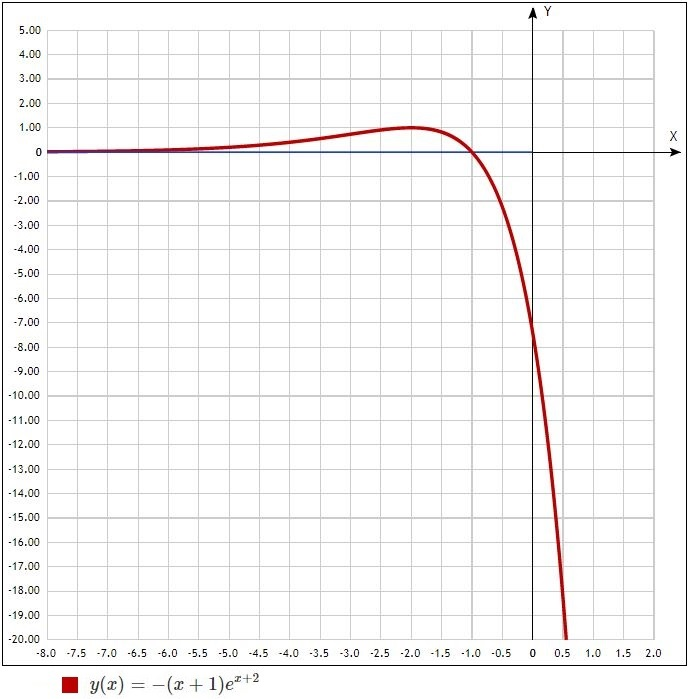
\includegraphics[width=\linewidth]{sol33}\end{figure}\end{minipage}
\end{minipage}\vspace{-4mm}}
{См. график.}{Выполнить все действия по схеме полного исследования функции.}
\end{problem}

\begin{problem}{Взятие производной для экспонент и логарифмов.}{11.2.8}{10A red мб построение графиков не типичных функций (10512) }{*}
{Провести полное исследование функции $y(x) = \displaystyle e^{\frac{1}{2 - x}}$, нарисовать её график.}
{Дробь в показателе экспоненты не определена при $x = 2$, а во всех остальных точках $y(x)$ определена и непрерывна, поэтому область определения $D(y) = \mathbb{R}\backslash\{2\}$.\smallskip\\
Чётной/нечётной функция $y(x)$ не является, поэтому никаких симметрий нет.\smallskip\\
У $y(x)$ есть точка разрыва в $x = 2$. Проверим, что с вертикальными асимптотами, для этого вычислим односторонние пределы $\lim\limits_{x\to 2+} y(x)$ и $\lim\limits_{x\to 2-} y(x)$.\\
$\displaystyle \lim\limits_{x\to 2+} y(x) = \lim\limits_{x\to 2+} e^{\frac{1}{2 - x}} = \lim\limits_{t\to 0+} e^{\frac{1}{-t}} = \lim\limits_{M\to -\infty} \!\!e^{M} = 0$.\\
$\displaystyle \lim\limits_{x\to 2-} y(x) = \lim\limits_{x\to 2-} e^{\frac{1}{2 - x}} = \lim\limits_{t\to 0-} e^{\frac{1}{-t}} = \lim\limits_{M\to +\infty} \!\!e^{M} = +\infty$.\\
Таким образом, вертикальная прямая $x = 2$ является асимптотой, но только для левой части графика. Правая же часть графика стартует из выколотой точки $(2; 0)$, тут асимптоты нет.\smallskip\\
Точки пересечения $y(x)$ с осью абсцисс отсутствуют: $e^t \neq 0$ для любых $t$.\smallskip\\
Так как $y(x)$ является показательной функцией, $y(x) > 0$ при $x \in D(y)$. \smallskip\\
Найдем критические точки функции $y(x)$. Для этого решим уравнение $y'(x) = 0$:\\ $\displaystyle y'(x) = \left(e^{\frac{1}{2 - x}}\right)' = e^{\frac{1}{2 - x}} \cdot \left(\tfrac{1}{2 - x}\right)' = e^{\frac{1}{2 - x}} \cdot \frac{-(-1)}{(2 - x)^2} = \frac{e^{\frac{1}{2 - x}}}{(x - 2)^2} = 0 \;\Rightarrow\; x \in \varnothing$.\\ То есть, у функции $y(x)$ нет критических точек (а значит, и локальных минимумов/максимумов тоже нет)\smallskip\\
Теперь находим промежутки возрастания и убывания:\\ $\displaystyle y'(x) = \frac{e^{\frac{1}{2 - x}}}{(x - 2)^2} >0$, поэтому $y(x)$ возрастает на всей своей области определения.\vspace{-3mm}\\
\begin{minipage}{\linewidth}
    \begin{minipage}{0.45\linewidth}
Проверим наличие горизонтальных/ наклонных асимптот у $y(x)$, вначале находим $k$: $\,k = \displaystyle \lim\limits_{x\to \pm\infty}\!\frac{y(x)}{x} =$ \\$\displaystyle = \lim\limits_{x\to \pm\infty}\!\frac{e^{\frac{1}{2 - x}}}{x} = \lim\limits_{x\to \pm\infty}\!\frac{e^{0}}{x} =0$.\medskip\\ Теперь $b$: $\,\displaystyle b = \!\lim\limits_{x\to \pm\infty}(y(x) - kx) =$\\ $\displaystyle =\lim\limits_{x\to \pm\infty}\!e^{\frac{1}{2 - x}} = e^0 = 1$.\\ Поэтому прямая $y = 1$ является \\горизонтальной асимптотой.\bigskip\\
Область значений $E(y) = (0; +\infty)$.\bigskip\\
График функции $y(x) = e^{\frac{1}{2 - x}}$ изображён на рисунке справа:
    \end{minipage}
    \hspace{0.02\linewidth}
    \begin{minipage}{0.53\linewidth}\begin{figure}[H] 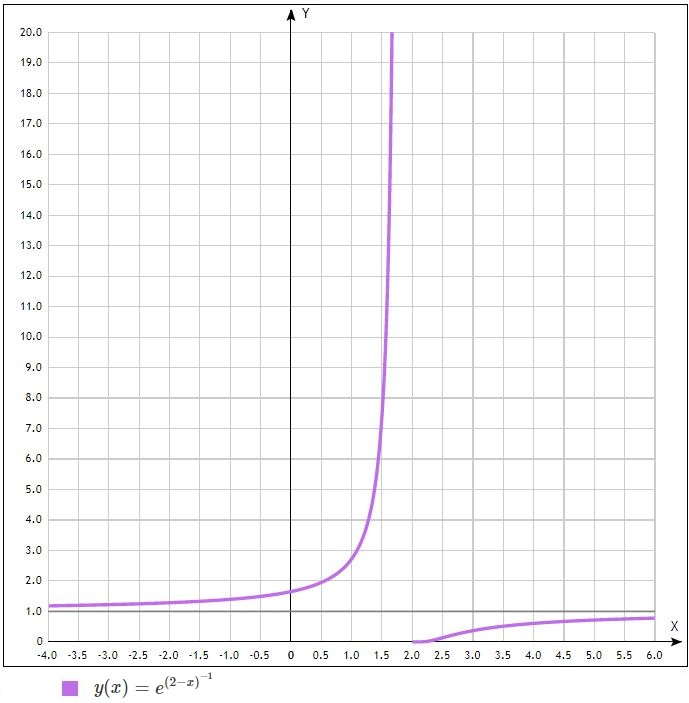
\includegraphics[width=\linewidth]{sol34}\end{figure}\end{minipage}
\end{minipage}\vspace{-4mm}}
{См. график.}{Выполнить все действия по схеме полного исследования функции.}
\end{problem}

\end{document}